%!TEX encoding = UTF-8 Unicode
% -*- coding: UTF-8; -*-
% vim: set fenc-utf-8

\chapter{Diagramme d'activité}
\label{s:diagramme_activite}

\begin{figure}[htpb]
    \centering
    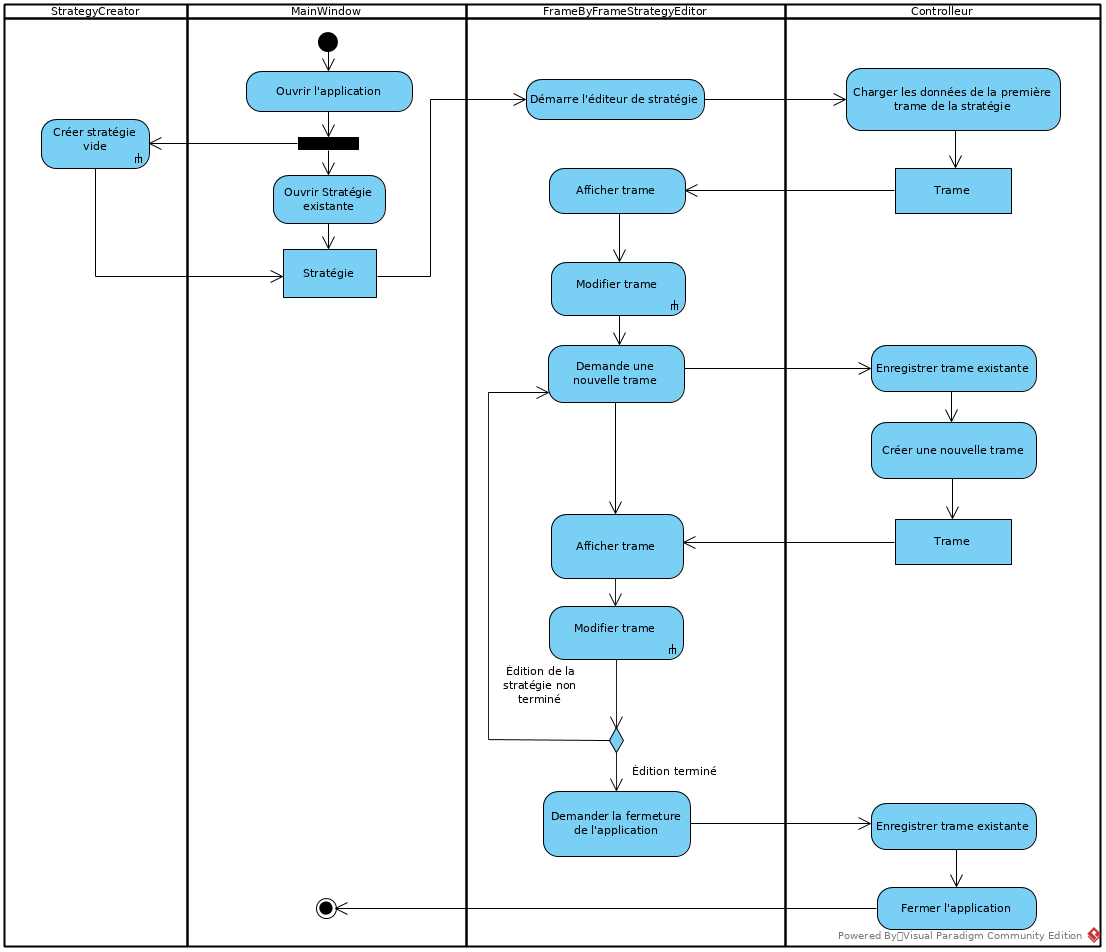
\includegraphics[scale=0.60]{fig/activity_diagram_imagepimage.png}
    \caption{Diagramme d'activité de la création d'une stratégie en mode image par image}
    \label{fig:activity_diagram_imagepimage}
\end{figure}

La figure \ref{fig:activity_diagram_imagepimage} représente le diagramme d'activité lors de l'édition de la stratégie en mode image par image.
L'initialisation de l'édition d'une stratégie se fait lors de la création ou de l'ouverture de celle-ci.
L'édition va toujours commencer sur la première trame.
La figure \ref{fig:sub_activity_diagram_create_strategy} représente le diagramme de sous-activité de la création d'une stratégie vide.
L'option \textit{Activer le nombre maximum de joueurs par équipe} va, lors de l'édition, empêcher l'utilisateur de placer un nombre de joueurs plus grand que le maximum permi par le sport.
L'option \textit{Activer le nombre maximum d'équipes} va, lors de l'édition, empêcher l'utilisateur de placer sur le terrain plus d'équipes que le maximum permis par le sport.
La figure \ref{fig:sub_activity_diagram_edit_strategy} représente le diagramme de sous-activité de l'édition d'une trame d'une stratégie.
Tel que mentionnée dans le diagramme d'état d'un joueur, en \ref{sec:diagramme_etat_joueur}, le nombre de joueur pouvant avoir le projectile est limité au nombre de projectiles.

\begin{figure}[htpb]
    \centering
    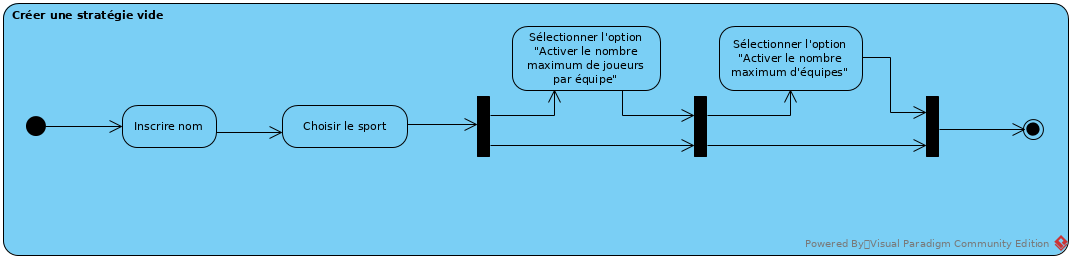
\includegraphics[scale=0.60]{fig/sub_activity_diagram_create_strategy.png}
    \caption{Diagramme de sous-activité de la création d'une stratégie vide}
    \label{fig:sub_activity_diagram_create_strategy}
\end{figure}

\begin{figure}[htpb]
    \centering
    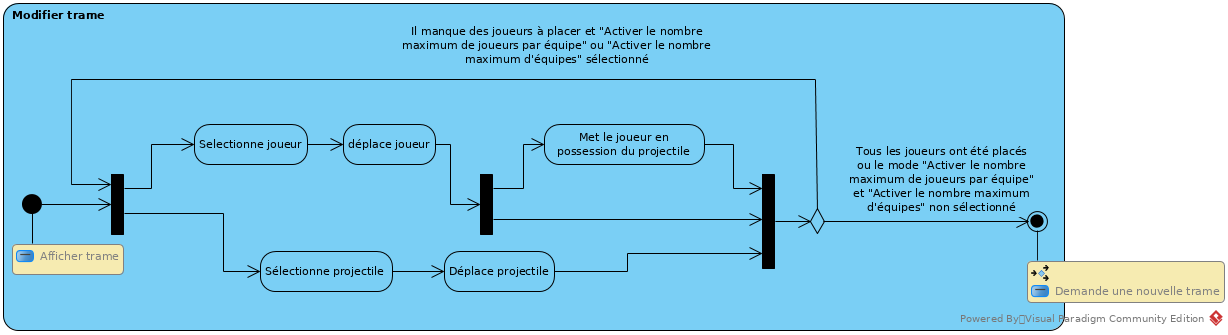
\includegraphics[scale=0.60]{fig/sub_activity_diagram_edit_strategy.png}
    \caption{Diagramme de sous-activité de l'édition d'une trame d'une stratégie}
    \label{fig:sub_activity_diagram_edit_strategy}
\end{figure}
